\documentclass{article}\usepackage{amsmath,amssymb,amsthm,tikz,tkz-graph,color,chngpage,soul,hyperref,csquotes,graphicx,floatrow}\newcommand*{\QEDB}{\hfill\ensuremath{\square}}\newtheorem*{prop}{Proposition}\renewcommand{\theenumi}{\alph{enumi}}\usepackage[shortlabels]{enumitem}\usepackage[nobreak=true]{mdframed}\usetikzlibrary{matrix,calc}\MakeOuterQuote{"}\usepackage[margin=0.75in]{geometry} \newtheorem{theorem}{Theorem}
\usepackage{listings}
\usepackage{color}
\usepackage{listings}
\usepackage{lstautogobble}
\usepackage{fancyvrb}
\lstset{basicstyle=\ttfamily,
  mathescape=true,
  escapeinside=||,
  autogobble}

\title{Problem Set 7}
\author{Name: $\quad$SID: }
\date{Spring 2016$\quad$GSI: }
\begin{document}
\maketitle

\section*{Warmup}

%%%% Problem 1 %%%%
\subsection*{1. Correcting XYZ}
\begin{enumerate}
\item For any java program, $P$, define $S(P)$ to be the set of all Java programs $P'$ that output the same result as $P$ on all inputs. Formally, $S(P)=\{P'\mid\forall x:P(x)=P'(x)$, $P'(x)$ \text{ halts if and only if } $P(x)$ \text{ halts}$\}$. XYZ claims that they have built an optimal java-program-shortner. Formally, they claim to have a procedure \textbf{optimalShortner} such that:
\begin{center}
\begin{BVerbatim}
for every java program P:
    let P' = optimalShortner(P)
    then:
        P' is in S(P)
        for all P'' in S(P), length(P'') >= length(P')
\end{BVerbatim}
\end{center}
Prove that XYZ is wrong.
\begin{mdframed}
\textbf{Solution}
% Solution here

\end{mdframed}
\item Having failed with source code shortening, XYZ now tries their luck with runtime optimization. XYZ claims that they have built a new optimizer \textbf{optimizer} such that:
\begin{center}
\begin{BVerbatim}
for every java program P:
    let P' = optimizer(P)
    then:
        forall x:
            if P(x) halts
            then P'(x) halts within 2^{|x|} steps
            else P'(x) infinite loops
\end{BVerbatim}
\end{center}
Namely, XYZ claims that their optimizer outputs an equivalent program such that: if $P(x)$ halts, then $P'(x)$ will halt within $2^{|x|}$ steps; if $P(x)$ does not halt, then $P'(x)$ does not halt either. Prove that \textbf{optimizer} can not exist.
\begin{mdframed}
\textbf{Solution}
% Solution here

\end{mdframed}
\item Let XYZ-phone be a smart phone with 16GB of storage, 2GB of RAM, and additional state of 1MB (i.e. CPU registers, etc).

\vspace{1mm}

\noindent Prove that for any program $P$ which does not interact with the rest of the world (no user input, no network connection, no wifi, no bluetooth, no sensors), it is possible to determine whether all executions of $P$ halts or whether some execution of $P$ infinite loops. (Different executions of $P$ may behave differently due to the random number generator, the initial state of the phone when $P$ is loaded, and due to non-determinism caused by multi-threading.
\begin{mdframed}
\textbf{Solution}
% Solution here

\end{mdframed}
\end{enumerate}

\clearpage

%%%% Problem 2 %%%%
\subsection*{2. Printing all $x$ where $M(x)$ halts}
Prove that it is possible to write a program $P$ which:
\begin{center}
\begin{BVerbatim}
* takes as input M, a java program
* runs forever, and prints out strings to the console
* for every x, if M(x) halts, then P(M) eventually prints out x
* for every x, if M(x) does NOT halt, then P(M) never prints out x
\end{BVerbatim}
\end{center}
\begin{mdframed}
\textbf{Solution}
% Solution here

\end{mdframed}
\clearpage

%%%% Problem 3 %%%%
\subsection*{3. Lexicographical output is impossible}
Lexicographical ordering of strings means (1) shorter strings are in front of longer strings (2) for two strings of the same length, they are sorted in alphabetical order.

\vspace{1mm}

\noindent Prove that it's impossible to solve the above problem if we require the output be in lexicographical order.
\begin{mdframed}
\textbf{Solution}
% Solution here

\end{mdframed}
\clearpage

%%%% Problem 4 %%%%
\subsection*{4. Maze}
Let's assume that Tom is located at the bottom left corner of the maze below, and Jerry is located at the top right corner. Tom of course wants to get to Jerry by the shortest path possible.
\begin{center}
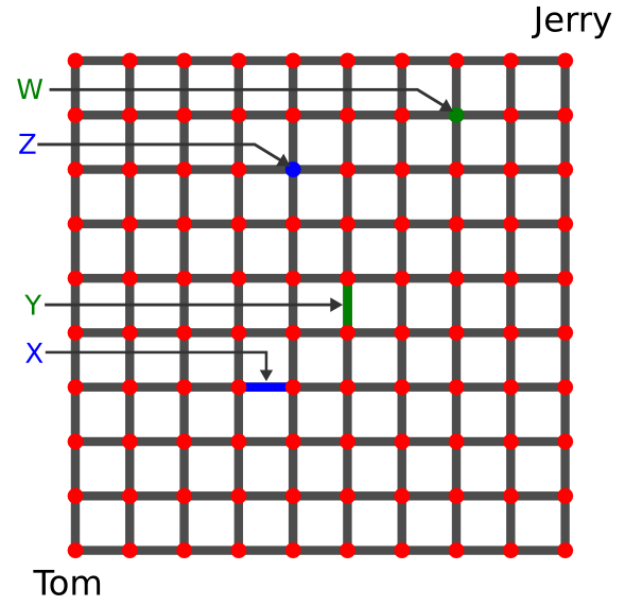
\includegraphics[scale=0.3]{graph}
\end{center}
\begin{enumerate}
\item How many such shortest paths exist?
\begin{mdframed}
\textbf{Solution}
% Solution here

\end{mdframed}
\item How many shortest paths pass through the edge labelled $X$? The edge labelled $Y$? Both the edges $X$ and $Y$? Neither edge $X$ nor edge $Y$?
\begin{mdframed}
\textbf{Solution}
% Solution here

\end{mdframed}
\item How many shortest paths pass through the vertex labelled $Z$? The vertex labelled $W$? Both the vertices $Z$ and $W$? Neither vertex $Z$ nor vertex $W$?
\begin{mdframed}
\textbf{Solution}
% Solution here

\end{mdframed}
\end{enumerate}
\clearpage

%%%% Problem 5 %%%%
\subsection*{5. Counting Practice!}
The only way to learn counting is to practice, practice, practice -- so here is your chance to do so. No need to justify your answers or show your calculations on this problem. We encourage you to leave your answer as an expression (rather than trying to evaluate it to get a specific number).
\begin{enumerate}
\item How many $10$-bit strings are there that contain exactly $4$ ones?
\begin{mdframed}
\textbf{Solution}
% Solution here

\end{mdframed}
\item How many different $13$-card bridge hands are there? (A bridge hand is obtained by selecting $13$ cards from a standard $52$-card deck. The order of the cards in a bridge hand is irrelevant.)
\begin{mdframed}
\textbf{Solution}
% Solution here

\end{mdframed}
\item How many different $13$-card bridge hands are there that contain no aces?
\begin{mdframed}
\textbf{Solution}
% Solution here

\end{mdframed}
\item How many different $13$-card bridge hands are there that contain all four aces?
\begin{mdframed}
\textbf{Solution}
% Solution here

\end{mdframed}
\item How many different $13$-card bridge hands are there that contain exactly $6$ spades?
\begin{mdframed}
\textbf{Solution}
% Solution here

\end{mdframed}
\item How many $99$-bit strings are there that contain more ones than zeros?
\begin{mdframed}
\textbf{Solution}
% Solution here

\end{mdframed}
\item If we have a standard $52$-card deck, how many ways are there to order these $52$ cards?
\begin{mdframed}
\textbf{Solution}
% Solution here

\end{mdframed}
\item Two identical decks of $52$ cards are mixed together, yielding a stack of $104$ cards. How many different ways are there to order this stack of $104$ cards?
\begin{mdframed}
\textbf{Solution}
% Solution here

\end{mdframed}
\item How many different anagrams of FLORIDA are there? (An anagram of FLORIDA is any reordering of the letters of FLORIDA, i.e., any string made up of the letters F, L, O, R, I, D, and A, in any order. The anagram does not have to be an English word.)
\begin{mdframed}
\textbf{Solution}
% Solution here

\end{mdframed}
\item How many different anagrams of ALASKA are there?
\begin{mdframed}
\textbf{Solution}
% Solution here

\end{mdframed}
\item How many different anagrams of ALABAMA are there?
\begin{mdframed}
\textbf{Solution}
% Solution here

\end{mdframed}
\item How many different anagrams of MONTANA are there?
\begin{mdframed}
\textbf{Solution}
% Solution here

\end{mdframed}
\item We have $9$ balls, numbered $1$ through $9$, and $27$ bins. How many different ways are there to distribute these $9$ balls among the $27$ bins?
\begin{mdframed}
\textbf{Solution}
% Solution here

\end{mdframed}
\item We throw $9$ identical balls into $7$ bins. How many different ways are there to distribute these $9$ balls among the $7$ bins such that no bin is empty?
\begin{mdframed}
\textbf{Solution}
% Solution here

\end{mdframed}
\item How many different ways are there to throw $9$ identical balls into $27$ bins?
\begin{mdframed}
\textbf{Solution}
% Solution here

\end{mdframed}
\item There are exactly $132$ students currently enrolled in CS70. How many different ways are there to pair up the $132$ CS70 students, so that each student is paired with one other student?
\begin{mdframed}
\textbf{Solution}
% Solution here

\end{mdframed}
\item How many ways are there to arrange $n$ $1$s and $k$ $0$s into a sequence?
\begin{mdframed}
\textbf{Solution}
% Solution here

\end{mdframed}
\item How many solutions does $$x_0+x_1+\ldots+x_k=n$$ have, if all $x$'s must be non-negative integers?
\begin{mdframed}
\textbf{Solution}
% Solution here

\end{mdframed}
\item How many solutions does $$x_0+x_1=n$$ have, if all $x$'s must be \textit{strictly positive} integers?
\begin{mdframed}
\textbf{Solution}
% Solution here

\end{mdframed}
\item How many solutions does $$x_0+x_1+\ldots+x_k=n$$ have, if all $x$'s must be \textit{strictly positive} integers?
 \begin{mdframed}
\textbf{Solution}
% Solution here

\end{mdframed}
\end{enumerate}
\clearpage

%%%% Problem 6 %%%%
\subsection*{6. Prove the following identities by combinatorial argument:}
\begin{enumerate}
\item $${n\choose k}= {{n-1}\choose {k-1}} + {{n-1}\choose k}$$
\begin{mdframed}
\textbf{Solution}
% Solution here

\end{mdframed}
\item $${{2n}\choose 2}=2{n\choose 2}+n^2$$
\begin{mdframed}
\textbf{Solution}
% Solution here

\end{mdframed}
\item $$\sum_{k=0}^nk{n\choose k}=n2^{n-1}$$
\begin{mdframed}
\textbf{Solution}
% Solution here

\end{mdframed}
\item $$\sum_{k=j}^n{n\choose k}{k\choose j}=2^{n-j}{n\choose j}$$
\begin{mdframed}
\textbf{Solution}
% Solution here

\end{mdframed}
\item $$\sum_{i=0}^k{m\choose i}{n\choose{k-i}}={{m+n}\choose k}$$
\begin{mdframed}
\textbf{Solution}
% Solution here

\end{mdframed}
\end{enumerate}
\clearpage

\end{document}